\subsection[]{Grundlagen}

\begin{frame}{Szintillatoren}

\begin{description}
	  \item[Szintillatoren] bestehen aus Material, dessen Moleküle nach Anregung durch geladene
	  Teilchen oder Photonen die Anregungsenergie in Form von Licht wieder abgeben
	\end{description}
	\begin{block}{Arten}
		\begin{itemize}
		  \item organische Szintillatoren (Kristalle, Gläser, Edelgase)
		  \item anorganische Szintillatoren (Kristalle, Flüssigkeiten, Plastik)
		\end{itemize}
	\end{block}
	\vspace{0.7cm}
	Auslese i.d.R. durch Photomultiplier
\end{frame}	


\begin{frame}{Szintillatoren}
	\begin{block}{Anorganische Szintillatoren}
		\begin{itemize}
		  \item anorganische Kristalle mit eingebrachten Fremdatomen (Aktivatorzentren) $\rightarrow$
		  zusätzliche Energieniveaus
		  \item durch eintreffende Strahlung angeregtes $e^-$ wandert durch Kristall, bis es auf Loch
		  trifft und rekombiniert $\rightarrow$ Abgabe eines Photons
		  \item Bsp.: NaI,CsI, BaF$_2$,
		\end{itemize}
	\end{block}
		\begin{block}{Organische Szintillatoren}
		\begin{itemize}
		  \item aromatische Kohlenwasserstoffverbindungen
		  \item hauptsächlich organische Kristalle oder Plastikszintillatoren
		  \item 
		  \item Bsp.: C$_{10}$H$_8$, C$_{14}$H$_{10}$
		\end{itemize}
	\end{block}
\end{frame}	

	
\subsection[]{Szintillationszähler}



\begin{frame}{Szintillationszähler}
	\begin{columns}[T]
		\column{.45\textwidth}
			\begin{itemize}
			  \item Bündelung von Szintillationsfasern ($\varnothing~<$~1~mm)
			  \item oft 1-2 Mäntel um Fasern, um Lichtausbeute zu erhöhen
			  \item Anordnung der Faser je nach Detektorgeometrie
			\end{itemize}	
	    \column{.5\textwidth}
	    	\begin{figure}[htbp]
			  \centering
			  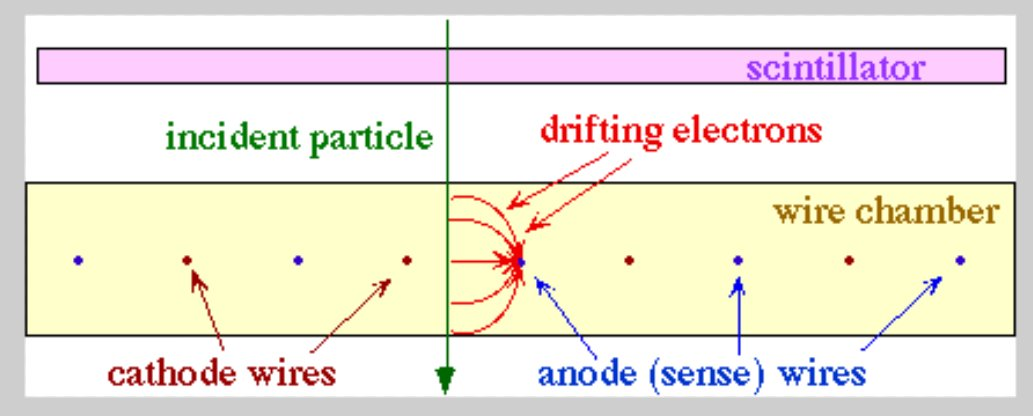
\includegraphics[width=\textwidth]{drift.gif}
% 			  \caption{Aufbau eines Szintillationszählers}
			\end{figure}
    \end{columns}
\end{frame}	
	
	\begin{frame}{Szintillationszähler}
    \begin{columns}[T]
		\column{.45\textwidth}
			Vorteile		
			\vspace{0.7cm}
			\begin{itemize}
			  \item 
			\end{itemize}	
	    \column{.5\textwidth}
	    	Nachteile
	    	\vspace{0.7cm}
	    	\begin{itemize}
			  \item 
			\end{itemize}
    \end{columns}
\end{frame}